\documentclass[margin=3mm]{standalone}
\usepackage{tikz}
\usetikzlibrary{patterns}
\begin{document}
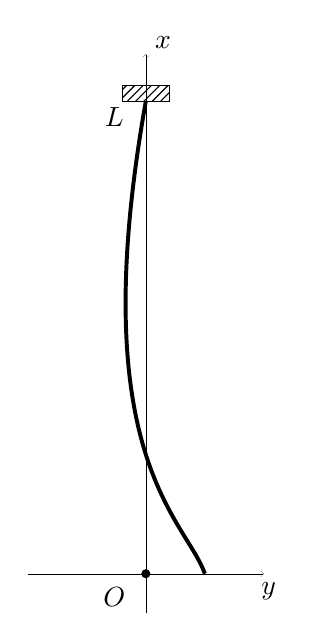
\begin{tikzpicture}
    \draw [line width = 0.01mm, ->] (0, 0) -- (3, 0) node [below, pos=1.02] {$y$};
    \draw [line width = 0.01mm , ->] (1.5, -0.5) -- (1.5, 6.6) node [right, pos=1.02] {$x$};
    \node at (1.1, 5.8) {$L$};
    \draw [pattern=north east lines] (1.2, 6) rectangle (1.8, 6.2);
    \node at (1.1, -0.3) {$O$};
    \draw [fill] (1.5, 0) circle (0.05);
    % \draw [fill, color=blue] (2, 0.7) circle (0.05);
    % \draw [fill, color=red] (0.7, 1.5) circle (0.05);
    \draw [line width = 0.5mm] (2.25, 0) .. controls (2, 0.7) and (0.7, 1.5) .. (1.5, 6);
\end{tikzpicture}
\end{document}